\documentclass[12pt,a4paper]{article}

\usepackage[a4paper, left=2.5cm, right=2.5cm, top=3cm, bottom=3cm]{geometry}  
\usepackage[brazil]{babel}  
\usepackage{float}  
\usepackage{csquotes}
\usepackage{setspace}       
\usepackage{graphicx}       
\usepackage{amsmath}        
\usepackage{hyperref}       
\usepackage{cleveref} 
\usepackage{lipsum}         
\usepackage{textcomp}       
\usepackage{booktabs}  
\usepackage{array}     
\usepackage{amssymb}
\usepackage{bookmark} 
\usepackage[utf8]{inputenc}
\usepackage[
     date=year,
     backend=biber,
     backref=page,
     style=numeric-comp,
     bibstyle=ieee,
     url=false,
     isbn=true,
     sorting=nty,
     sortcites=true
]{biblatex}
\usepackage{url}
\usepackage{xurl}
	 
\doublespacing

 \AtEveryBibitem{\clearfield{pages}}
 \AtEveryBibitem{\clearfield{notes}}

\addbibresource{ic.bib}

\title{\Large{Relatório de Estudo Dirigido} \\ \textbf{Otimização Combinatória para Geração de Árvores de Decisão}}
\author{Aluna: Sofia Valverde Villas Bôas\\
    RA 252974 - Engenharia de Computação AA\\
    s252974@dac.unicamp.br
\\ Orientador: Prof.\ Dr.\ Rafael Crivellari Saliba Schouery}
\date{}

\begin{document}

\maketitle

\section{Introdução} \label{sec:introducao}

Suponha que um laboratório necessite estimar a eficácia de um medicamento em desenvolvimento, considerando características como idade, sexo e dosagem receitada para os indivíduos. Uma forma de abordar este problema é por meio de \emph{árvores de decisão}, técnica utilizada para categorização de dados em classes \cite{}. No exemplo, cada classe está relacionada a um grau de eficácia do medicamento. A categorização ilustrada na \autoref{fig:arvore-exemplo} ocorre via uma série de perguntas, representadas pelos retângulos, referentes às características do conjunto de dados. 

\begin{figure}[H]
    \centering
    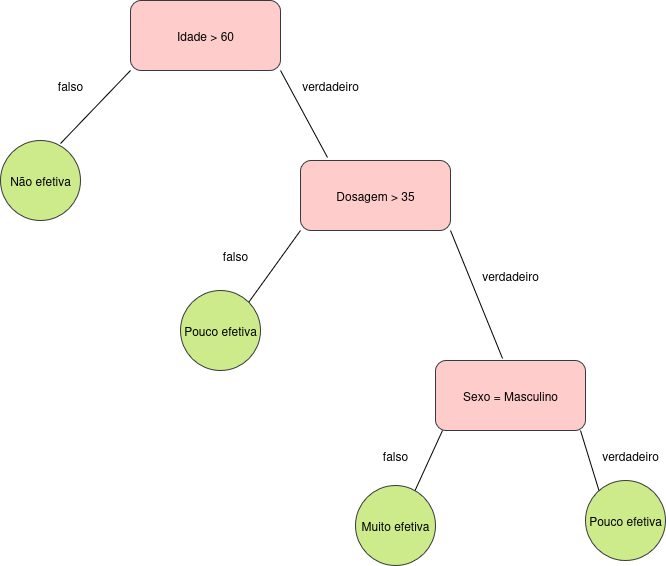
\includegraphics[width=0.7\textwidth, height=12cm]{Decision Tree V2.png}
    \caption{Árvore de decisão para fabricação de um medicamento hipotético. Nós internos (retângulos) da árvore representam perguntas aplicadas a características dos dados. As ligações ("verdadeiro" ou "falso") correspondem ao caminho a seguir dependendo do resultado da pergunta. Os nós folhas são classes alvo do problema, isto é, os níveis de eficácia do medicamento.}
    \label{fig:arvore-exemplo}
\end{figure}

Uma vantagem associada a estas árvores é a facilidade de extrair informações relevantes, conceito chamado de \emph{explicabilidade} \cite{Bertsimas2017, Costa2022, Rudin2019}. Assim, estas árvores evidenciam quais atributos foram mais importantes para a tomada de decisão. Por exemplo, o medicamento funciona eficientemente para pacientes do sexo masculino, com até 60 anos e que receberam dosagem acima de 35. Este agrupamento facilita a interpretação do modelo e a obtenção de novas hipóteses.

Algoritmos para geração de \emph{árvores de decisão} tradicionalmente as constroem de forma heurística, realizando recursivamente escolhas locais ótimas em cada nó \cite{Costa2022}. Apesar de obter resultados razoáveis na prática \cite{Linden2024}, este processo pode deixar de capturar pontos essenciais dos \textit{datasets} \cite{Bertsimas2017}.

Em 2017, Bertsimas e Dunn \cite{Bertsimas2017} propuseram a possibilidade de gerar árvores de decisão \emph{ótimas}. Ao construir globalmente a árvore que melhor representa os dados, esta técnica permite aliar explicabilidade e precisão na categorização. 

Contudo, o problema de gerar árvores ótimas é NP-Difícil \cite{Hyafil1976}, ou seja, não se conhecem algoritmos que o resolvam em tempo polinomial. Esta complexidade contrasta com o potencial de aplicação destes modelos na resolução de problemas práticos, como no cálculo de risco em cirurgias de emergência \cite{Bertsimas2018}, no aumento da segurança dinâmica em sistemas de energia elétrica \cite{Genc2010} ou na recomendação de políticas sociais \cite{Chan2019}. Apesar de difícil, o impacto do uso deste método evidencia a necessidade de desenvolver algoritmos computacionalmente eficazes. 

Portanto, o objetivo principal deste estudo dirigido consiste no estudo de técnicas de Programação Linear Inteira (PLI) para a formulação do problema, em paralelo com a leitura de artigos sobre modelos e funcionamento de árvores de decisão. A partir disso, partiu-se para o estudo da otimalidade nestas árvores, bem como a análise do impacto de possíveis formulações e características a serem otimizadas. Além disso, buscou-se introduzir a aluna às práticas acadêmicas, contribuindo para sua formação e eventual iniciação científica.

\section{Atividades Previstas} \label{sec:atividades-previstas}

O primeiro passo consistiu no estudo mais aprofundado de Programação Linear Inteira, baseando-se especialmente nos livros de Wolsey \cite{Wolsey2021} e Chvátal \cite{Chvatal1983}. Paralelamente, a aluna também aprofundou os conhecimentos sobre árvores de decisão, de modo a conseguir perceber nuances, limitações e potencialidades desses modelos em diferentes contextos.

Em seguida, deu-se a análise de como PLI pode ser utilizada para otimizar características relevantes em árvores de decisão. Artigos que exploram essas aplicações como \cite{Verwer2019, Aghaei2021, Costa2022} foram analisados, destacando abordagens que formalizam a construção da árvore ótima como um problema de otimização inteira, permitindo controlar a complexidade, a explicabilidade e a justiça do modelo \cite{Bertsimas2017}.

\section{Resultados} \label{sec:resultados}

Em seguida, são apresentados os principais tópicos estudados ao longo do período do estudo dirigido.

\subsection{Programação Linear Inteira}
Falar que aprendi os fundamentos das técnicas que vou usar na IC

- PL e simplex
- PLI, dualidade, convex hull, branch and bound, cutting plane...

\subsection{Árvores de Decisão Ótimas}

- possíveis formulações.

\subsection{Implementações e Experimentos}

Falar que aprendi a mexer no GUROBI, me familiarizando com o solver através da implementação de um modelo simples.

\section{Conclusão}

Durante o Estudo Dirigido, diversos aspectos colaboraram para o amadurecimento profissional e acadêmico da aluna. 
Entre eles, é importante mencionar a construção de uma base de conhecimentos em Programação Linear Inteira.
Através tanto do estudo individual, como das reuniões do grupo de pesquisa semanais, a aluna consolidou o entendimento de técnicas de PLI e como elas são aplicadas no contexto de otimização.

Além disso, a leitura de artigos sobre árvores de decisão ótimas colaborou para a compreensão do contexto de uso dessa técnica de categorização...

- Matérias do curso que eu usei:

* MC358, MC458, MC558
* Combinatória Poliédrica


\begingroup
\onehalfspacing
\printbibliography
\endgroup

\end{document}
